\RequirePackage[T1]{fontenc}
\documentclass[conference]{IEEEtran}
\usepackage{amsmath,amssymb}
\usepackage{booktabs}
\usepackage{cite}
\usepackage{graphicx}
\usepackage{url}

% Generated by run_all.py from results/. Edits will be overwritten.
\newcommand{\MatrixSize}{100}
\newcommand{\TrueRank}{5}
\newcommand{\Seed}{43}
\newcommand{\Trials}{5}
\newcommand{\Magnitude}{10}
\newcommand{\Threshold}{1}
\newcommand{\LambdaValue}{0.100}
\newcommand{\PenaltyScale}{0.3}
\newcommand{\StopTolerance}{1\times10^{-7}}
\newcommand{\IterationCap}{5000}
\newcommand{\MainTrialCount}{25}
\newcommand{\CorruptTrialCount}{20}
\newcommand{\CorruptWins}{20}
\newcommand{\GapTrend}{increases at every density step}
\newcommand{\MainConverged}{25}
\newcommand{\NoiseConverged}{15}
\newcommand{\NoiseTrials}{15}
\newcommand{\CleanPca}{1.44\times10^{-15}}
\newcommand{\CleanPcp}{2.81\times10^{-8}}
\newcommand{\EndPca}{2.116}
\newcommand{\EndPcp}{1.67\times10^{-7}}
\newcommand{\MainMinIterations}{2}
\newcommand{\MainMaxIterations}{41}
\newcommand{\MeanPcaMs}{0.79}
\newcommand{\MeanPcpMs}{21.05}
\newcommand{\CleanFalsePos}{0}
\newcommand{\CorruptTotalPos}{18500}
\newcommand{\CorruptFalsePos}{0}
\newcommand{\CorruptFalseNeg}{0}
\newcommand{\PooledPrecision}{1.000}
\newcommand{\PooledRecall}{1.000}
\newcommand{\RepPca}{1.242}
\newcommand{\RepPcp}{7.46\times10^{-8}}
\newcommand{\RepRank}{5}
\newcommand{\RepIterations}{32}
\newcommand{\RepStatus}{converged}
\newcommand{\RepPrimal}{1.82\times10^{-8}}
\newcommand{\RepDual}{8.14\times10^{-8}}
\newcommand{\RepTp}{1000}
\newcommand{\RepFp}{0}
\newcommand{\RepFn}{0}
\newcommand{\NoisePcp}{0.363}
\newcommand{\NoiseFalsePos}{991}
\newcommand{\NoiseFalseNeg}{0}
\newcommand{\NoiseMildIterations}{808.8}
\newcommand{\NoiseHighIterations}{193.6}
\newcommand{\Environment}{Windows 11 on an Intel(R) Core(TM) Ultra 9 275HX CPU. Python 3.14.4, NumPy 2.4.4, SciPy 1.17.1, and Matplotlib 3.10.8.}
\newcommand{\ErrorRows}{%
0\% & $1.44\times10^{-15} \pm 6.02\times10^{-16}$ & $2.81\times10^{-8} \pm 2.64\times10^{-8}$ \\
2\% & $0.496 \pm 0.041$ & $2.90\times10^{-8} \pm 1.31\times10^{-8}$ \\
5\% & $0.885 \pm 0.048$ & $4.90\times10^{-8} \pm 3.48\times10^{-8}$ \\
10\% & $1.330 \pm 0.068$ & $7.86\times10^{-8} \pm 1.96\times10^{-8}$ \\
20\% & $2.116 \pm 0.089$ & $1.67\times10^{-7} \pm 4.64\times10^{-8}$ \\
}
\newcommand{\DiagnosticRows}{%
0\% & $\text{--}$ & 5/5 & 7.2 [2, 9] & 3.6 \\
2\% & $1.000$ & 5/5 & 25.6 [24, 27] & 19.8 \\
5\% & $1.000$ & 5/5 & 27.8 [27, 28] & 23.3 \\
10\% & $1.000$ & 5/5 & 32.2 [30, 35] & 26.4 \\
20\% & $1.000$ & 5/5 & 39.0 [38, 41] & 32.2 \\
}
\newcommand{\NoiseRows}{%
0.0 & $1.391$ & $6.87\times10^{-8}$ & 5.0 & $1.000$ \\
0.1 & $1.391$ & $0.076$ & 54.2 & $1.000$ \\
0.5 & $1.401$ & $0.363$ & 54.8 & $0.910$ \\
}

\graphicspath{{../figures/}}
\newcommand{\fro}[1]{\left\|#1\right\|_{\mathrm F}}
\newcommand{\svt}{\operatorname{SVT}}
\newcommand{\soft}{\operatorname{Soft}}

\title{Robust Low-Rank Matrix Recovery Under Sparse Corruptions: A Comparative Study of PCA and Principal Component Pursuit}
\author{\IEEEauthorblockN{Aashish M}
\IEEEauthorblockA{EP23BT005, Engineering Physics\\{IIT Dharwad}\\{ep23bt005@iitdh.ac.in}}}

\begin{document}
\maketitle

\begin{abstract}
Low-rank representations can preserve useful structure in high-dimensional data, yet a small number of large entrywise errors can dominate a least-squares fit. This study compares known-rank truncated singular value decomposition with principal component pursuit (PCP) for recovery of a latent matrix and localization of sparse corruptions. We generate $\MatrixSize\times\MatrixSize$ Gaussian-factor matrices of rank $\TrueRank$, inject uniformly located signed errors of magnitude $\Magnitude$ at five densities from 0\% to 20\%, and evaluate both methods on the same observations in each of $\Trials$ trials per density. At 20\% corruption, mean relative Frobenius error is $\EndPca$ for truncated SVD and $\EndPcp$ for PCP. PCP has lower error in \CorruptWins{} of \CorruptTrialCount{} trials with gross errors, and the solver meets both residual criteria in \MainConverged{} of \MainTrialCount{} main trials. At a threshold of $\Threshold$, the detector registers \CorruptFalsePos{} false positives and misses \CorruptFalseNeg{} of the \CorruptTotalPos{} true corruptions in those trials. In a paired dense-noise extension, PCP error reaches $\NoisePcp$ at noise standard deviation $0.5$. The comparison quantifies recovery gains under the sparse-error model alongside the cost of repeated decompositions and the loss of accuracy under dense noise.
\end{abstract}

\begin{IEEEkeywords}
Robust PCA, principal component pursuit, low-rank recovery, sparse corruption, alternating direction method of multipliers
\end{IEEEkeywords}

\section{Introduction}
Low-rank approximation represents a matrix using a small set of latent directions. This representation underlies dimensionality reduction, image compression, and modeling of coherent signals across repeated measurements \cite{jolliffe2002}. A standard least-squares fit is effective when the dominant directions of the observations describe the signal of interest. Entrywise contamination can break that correspondence. For example, a few strong anomalies can change the leading singular vectors and spread reconstruction error to entries where the original measurements were accurate.

In applications such as background subtraction, a slowly varying scene can be modeled by a low-rank matrix of frames, with foreground motion producing changes on a subset of pixels \cite{candes2011}. Related decompositions can isolate anomalous observations and gross errors in images. The decomposition itself is an identification problem. Both the clean signal and the corruptions are unknown, and either component can explain some of the same patterns. Principal component pursuit (PCP) resolves this ambiguity under structural conditions by penalizing rank and sparsity through convex surrogates.

We ask how accurately a known-rank truncated SVD and equality-constrained PCP recover a clean low-rank matrix as the density of high-amplitude errors increases. Hypothesis H1 is that PCP provides lower reconstruction error than truncated SVD under incoherent low-rank structure and random sparse corruption, with a widening advantage as corruption density rises. We compare paired recovery errors across a density sweep, inspect both fitted components on a prespecified observation, and quantify detection at a fixed entrywise threshold. A separate paired noise experiment probes how PCP behaves when the observations also contain dense Gaussian noise.

\section{Related Work}
Jolliffe \cite{jolliffe2002} describes PCA through successive directions of maximal variance. The singular value decomposition supplies those directions when applied to centered data. The low-rank approximation theorem of Eckart and Young \cite{eckart1936} gives a related result for general matrices, where truncating the singular spectrum minimizes the squared Frobenius residual at a specified rank.

Fazel \emph{et al.} \cite{fazel2001} motivated replacing matrix rank with the nuclear norm in optimization. Wright \emph{et al.} \cite{wright2009} applied convex penalties to the separation of a low-rank component and sparse errors. Cand\`es \emph{et al.} \cite{candes2011} established recovery guarantees for PCP under incoherence and sparsity conditions and demonstrated applications in video and image analysis. The model studied here is the entrywise decomposition from that work.

Singular value thresholding (SVT) is the proximal map of the nuclear norm and was developed as a computational primitive for matrix completion by Cai \emph{et al.} \cite{cai2010}. We use it within the alternating direction method of multipliers (ADMM), following the scaled formulation and stationarity diagnostics described by Boyd \emph{et al.} \cite{boyd2011}. Zhou \emph{et al.} \cite{zhou2010} extend PCP to allow a bounded dense residual. Their formulation motivates our examination of model mismatch in the equality-constrained solver.

\section{Mathematical Formulation}
\subsection{Low-Rank Approximation}
Let the observed matrix $M\in\mathbb R^{m\times n}$ have compact singular value decomposition $M=U\Sigma V^\top$, with the singular values in descending order. The baseline solves
\begin{equation}
  \hat L_{\mathrm{PCA}}
    \in\arg\min_{\operatorname{rank}(L)\le r}\fro{M-L}^2.
  \label{eq:svd_objective}
\end{equation}
The solution is $U_r\Sigma_r V_r^\top$ \cite{eckart1936}. With rows interpreted as samples, mean-centered PCA instead decomposes $M-\mathbf{1}\bar m^\top$, where $\bar m$ is the vector of column means. A rank-$r$ PCA reconstruction in the original coordinates adds $\mathbf{1}\bar m^\top$ to that centered fit. It is an affine model, whose reconstruction can have matrix rank $r+1$. We use uncentered SVD because the target is the raw low-rank matrix $L_0$ and the error is measured in its original coordinates. The subscript PCA denotes this matrix approximation baseline throughout.

\subsection{Principal Component Pursuit}
Suppose $M=L_0+S_0$, with $L_0$ low rank and $S_0$ sparse. PCP estimates both components via
\begin{equation}
  \min_{L,S}\ \|L\|_*+\lambda\|S\|_1
  \quad\text{subject to}\quad L+S=M,
  \label{eq:pcp}
\end{equation}
where $\|L\|_*=\sum_i \sigma_i(L)$ and $\|S\|_1=\sum_{ij}|S_{ij}|$. The nuclear norm favors a concentrated singular spectrum, and the elementwise penalty favors a small support. The fixed weight $\lambda=1/\sqrt{\max(m,n)}$ follows \cite{candes2011}. PCP estimates the rank through its objective and has access only to $M$.

Identifiability depends on the geometry of $L_0$ and the support of $S_0$. A matrix supported on a single entry is both sparse and rank one. If such a pattern occurs within the low-rank signal, the observations alone can support multiple decompositions. Incoherence limits concentration of the singular spaces on coordinate axes. In particular, it bounds the largest row leverage scores of the left and right singular vector matrices and constrains the concentration of their product $UV^\top$ \cite{candes2011}. Uniformly scattered corruptions reduce alignment with low-rank patterns. Exact recovery guarantees in this model require suitable bounds on rank, sparsity, and incoherence. The Gaussian factor construction gives rotationally invariant column spaces, while finite draws can still have unequal leverage scores.

\subsection{Scaled ADMM and Stopping Criteria}
Let $R=M-L-S$ and $X$ be the multiplier for $R=0$. With penalty $\mu>0$ and scaled multiplier $Y=X/\mu$, the augmented Lagrangian is
\begin{equation}
  \|L\|_*+\lambda\|S\|_1
  +\frac{\mu}{2}\fro{R+Y}^{2}-\frac{\mu}{2}\fro{Y}^{2}.
  \label{eq:lagrangian}
\end{equation}
We complete the square in the current primal block and minimize it with the other block fixed. Minimization in $L$ gives a nuclear norm proximal map. For $Z=U_Z\Sigma_Z V_Z^\top$, it preserves the singular vectors and applies $(\sigma_i(Z)-t)_+=\max(\sigma_i(Z)-t,0)$ to each singular value at threshold $t$. Minimization in $S$ separates entrywise, with proximal map $\soft_t(z)=\operatorname{sign}(z)(|z|-t)_+$. The updates are
\begin{align}
 L^{k+1}&=\svt_{1/\mu}(M-S^k+Y^k), \label{eq:l_update}\\
 S^{k+1}&=\soft_{\lambda/\mu}(M-L^{k+1}+Y^k), \label{eq:s_update}\\
 Y^{k+1}&=Y^k+M-L^{k+1}-S^{k+1}. \label{eq:y_update}
\end{align}
We initialize $S^0=Y^0=0$ and use $\mu=\PenaltyScale\sqrt{mn}/\fro{M}$ for nonzero $M$. The fixed penalty scales inversely with the root mean square entry magnitude. A zero input admits the zero solution directly.

The primal residual measures feasibility. To derive the dual residual, write the first-order conditions of the two proximal steps using the updated multiplier $X^{k+1}=\mu Y^{k+1}$. The sparse step gives $X^{k+1}\in\lambda\partial\|S^{k+1}\|_1$, and the low-rank step gives
\begin{equation}
 X^{k+1}+\mu(S^{k+1}-S^k)\in\partial\|L^{k+1}\|_*.
\end{equation}
Thus $\mu(S^{k+1}-S^k)$ measures the stationarity mismatch for the low-rank block. For nonzero $M$, the two monitored residuals are
\begin{align}
 \rho_{\mathrm p}^{k+1}&=\frac{\fro{M-L^{k+1}-S^{k+1}}}{\fro{M}}, \label{eq:primal}\\
 \rho_{\mathrm d}^{k+1}&=\frac{\mu\fro{S^{k+1}-S^k}}{\max(1,\fro{X^{k+1}})}. \label{eq:dual}
\end{align}
The algorithm requires both residuals to reach the stopping tolerance in Table~\ref{tab:settings}. Feasibility alone gives no bound on the stationarity mismatch or the ground-truth error. If the iteration cap is reached first, the final iterate is scored and flagged as unconverged.

\section{Experimental Methodology}
\subsection{Synthetic Observations and Controls}
We draw $A\in\mathbb R^{m\times r}$ and $B\in\mathbb R^{n\times r}$ with independent standard normal entries and set $L_0=AB^\top/\sqrt{r}$. Each entry of $L_0$ then has unit variance. For density $p$, we choose $k=\operatorname{round}(pmn)$ entries uniformly without replacement. Each receives an independent sign and fixed magnitude $\Magnitude$, yielding $S_0$. The true support is $\Omega=\{(i,j):(S_0)_{ij}\ne0\}$. The clean control uses $p=0$.

\begin{table}[!t]
\caption{Synthetic Study and Solver Settings}
\label{tab:settings}
\centering
\small
\begin{tabular}{@{}ll@{}}
\toprule
Setting & Value \\
\midrule
Dimensions and true rank & $\MatrixSize\times\MatrixSize$, $r=\TrueRank$ \\
Gross error density $p$ & $0\%,\,2\%,\,5\%,\,10\%,\,20\%$ \\
Gross error amplitude & $\pm\Magnitude$ \\
Trials per condition and seed & \Trials{}, \Seed{} \\
PCP weight $\lambda$ & $\LambdaValue$ \\
ADMM penalty $\mu$ & $\PenaltyScale\sqrt{mn}/\fro{M}$ \\
Residual tolerance and cap & $\StopTolerance$, \IterationCap{} iterations \\
Detection threshold $\tau$ & $\Threshold$ \\
Dense noise sweep at $p=10\%$ & $\sigma\in\{0,0.1,0.5\}$ \\
\bottomrule
\end{tabular}
\end{table}

Each main trial has its own random stream and a fresh draw of both factors and corruption. The two solvers receive the exact same $M$ within a trial. Across density conditions we generate new matrices, so comparisons of the algorithms are paired within each condition. The known true rank is supplied to truncated SVD to remove rank selection as a confound. PCP uses the same regularization rule and stopping criteria across all trials. For visualization we select the first draw at $p=10\%$ before examining the errors.

In the dense-noise extension we form $M=L_0+S_0+\sigma Z$, where the entries of $Z$ are independent standard normals and $p=10\%$. Each extension trial uses its own independent stream. Within a trial, all values of $\sigma$ use the same $L_0$, $S_0$, and $Z$, isolating the change in noise scale. Equality-constrained PCP still enforces $L+S=M$, so it must account for the dense perturbation in its two fitted components.

\subsection{Metrics and Reproducibility}
We evaluate both low-rank estimates by relative Frobenius error,
\begin{equation}
  E_L=\frac{\fro{\hat L-L_0}}{\fro{L_0}}.
  \label{eq:relative_error}
\end{equation}
We report the arithmetic mean and sample standard deviation across trials. Error above one indicates a deviation larger in Frobenius norm than the clean signal itself. The error uses $L_0$ as the reference, whereas the SVD objective uses $M$.

The support estimate is $\hat\Omega=\{(i,j):|\hat S_{ij}|>\tau\}$. Precision is $\mathrm{TP}/(\mathrm{TP}+\mathrm{FP})$, recall is $\mathrm{TP}/(\mathrm{TP}+\mathrm{FN})$, and F1 is $2\mathrm{TP}/(2\mathrm{TP}+\mathrm{FP}+\mathrm{FN})$ for trials with positive true support. The false-positive rate is $\mathrm{FP}/(\mathrm{FP}+\mathrm{TN})$. Precision is undefined when there are zero detections. At 0\% density we report recall and F1 as undefined and use the false-alarm counts and rate to describe the detector. Means of support scores give equal weight to trials where the score is defined.

NumPy \texttt{SeedSequence} spawns separate branches for the density and dense-noise experiments, and \texttt{default\_rng} initializes individual trial streams. We save all simulated inputs, the two estimates of $L_0$ and the PCP estimate of $S_0$ for the illustrative trial, per-trial metrics, and per-iteration residuals. NumPy computes the metrics and SciPy supplies a full economy SVD for both methods. Timing covers each solver call including the PCP residual history, with one BLAS thread requested and data generation, plotting, and file I/O outside the timer. The execution environment was \Environment{}

\section{Results and Discussion}
\subsection{Reconstruction Across Corruption Densities}

\begin{figure}[!t]
 \centering
 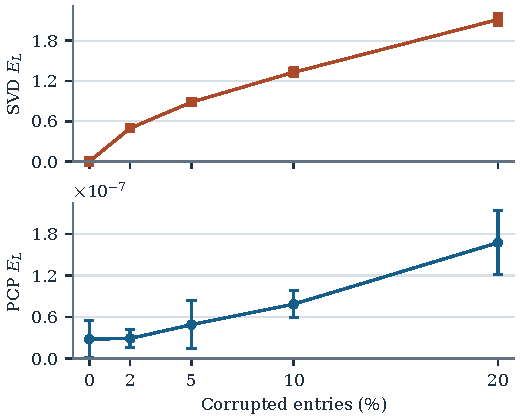
\includegraphics[width=\columnwidth]{reconstruction_error.pdf}
 \caption{Mean relative error across trials. The panels use separate vertical scales to show the variation in each method. Error bars show one sample standard deviation on each side, truncated at zero where needed.}
 \label{fig:errors}
\end{figure}

\begin{table}[!t]
\caption{Relative Low-Rank Error (Mean $\pm$ Sample SD)}
\label{tab:errors}
\centering
\small
\setlength{\tabcolsep}{4pt}
\begin{tabular}{@{}rcc@{}}
\toprule
$p$ & Truncated SVD & PCP \\
\midrule
\ErrorRows
\bottomrule
\end{tabular}
\end{table}

\begin{figure*}[!t]
 \centering
 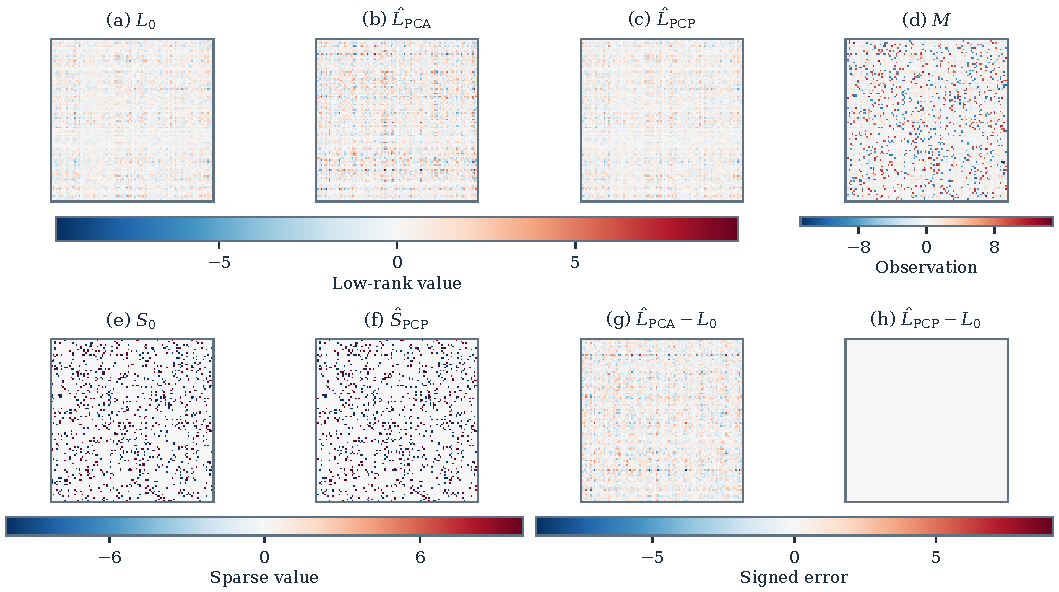
\includegraphics[width=\textwidth]{matrix_recovery.pdf}
 \caption{Prespecified 10\% corruption trial. Panels (a)--(c) use a common scale for the clean matrix and both reconstructions. Panel (d) shows the observation on its own scale. Panels (e) and (f) share a sparse-value scale. Panels (g) and (h) share a signed-error scale, so values near zero are rendered with the same color in both.}
 \label{fig:matrix}
\end{figure*}

Table~\ref{tab:errors} and Fig.~\ref{fig:errors} compare recovery at each density. In the clean control, the mean relative errors are $\CleanPca$ for SVD and $\CleanPcp$ for PCP. Truncation can recover a clean rank-$r$ matrix to floating-point precision, while PCP returns a solution subject to its numerical stopping rule. At 20\%, the mean errors are $\EndPca$ and $\EndPcp$, respectively. Across the corrupted observations, PCP yields lower error in \CorruptWins{} of \CorruptTrialCount{} paired comparisons. The difference in mean errors, SVD minus PCP, \GapTrend{}. These contrasts evaluate H1 descriptively. The standard deviations summarize variation over the sampled trials.

The energy of the sparse component is $\fro{S_0}^2=k\Magnitude^2$, whereas $\mathbb E[\fro{L_0}^2]=mn$. Thus the ratio of corruption norm to root mean square signal norm is $\Magnitude\sqrt{k/(mn)}$. The larger this ratio, the more the least-squares objective can benefit by spending rank on directions influenced by outliers. That objective rewards fitting the observed values, even at corrupted entries. The PCP penalty permits gross errors to be assigned directly to the sparse block, preserving the low-rank structure when the geometry allows a clean separation.

\subsection{Component Recovery and Support}
Figure~\ref{fig:matrix} illustrates the difference between fitting $M$ and recovering $L_0$. In the selected 10\% trial, the SVD and PCP errors are $\RepPca$ and $\RepPcp$. The rank retained by the last PCP thresholding step is \RepRank{}. Using identical color limits for the low-rank matrices and a separate common limit for the two error maps keeps the comparison on the same amplitude scale.

\begin{figure}[!t]
 \centering
 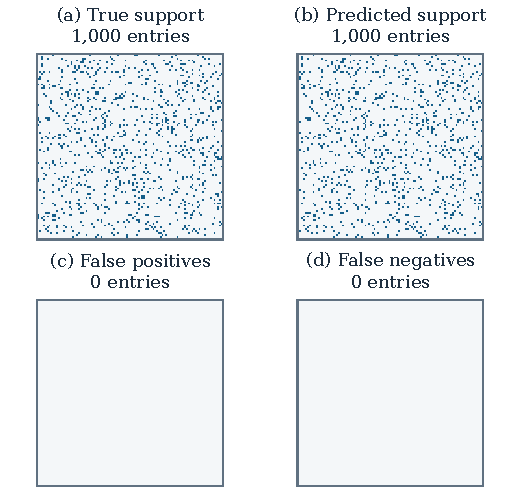
\includegraphics[width=0.94\columnwidth]{corruption_detection.pdf}
 \caption{Support of the sparse component in the 10\% trial. The predicted mask uses $|\hat S_{ij}|>\Threshold$. Colored cells mark membership in each mask. Counts include all entries in the panel.}
 \label{fig:support}
\end{figure}

\begin{table}[!t]
\caption{Support and PCP Solver Diagnostics by Density}
\label{tab:diagnostics}
\centering
\small
\setlength{\tabcolsep}{4pt}
\begin{tabular}{@{}rcccc@{}}
\toprule
$p$ & Mean F1 & Converged & Iter.\ mean [range] & Mean ms \\
\midrule
\DiagnosticRows
\bottomrule
\end{tabular}
\end{table}

Figure~\ref{fig:support} compares the true and estimated masks. The representative fit has \RepTp{} true detections, \RepFp{} false positives, and \RepFn{} false negatives. Across the corrupted observations there are \CorruptTotalPos{} true corrupted entries, \CorruptFalsePos{} false positives, and \CorruptFalseNeg{} false negatives. Pooling the entries across those trials gives precision $\PooledPrecision$ and recall $\PooledRecall$. The clean trials yield \CleanFalsePos{} false alarms and have undefined F1 (Table~\ref{tab:diagnostics}). The threshold is calibrated to a setting where corruptions have known and constant amplitude. With weaker or variable errors, a single amplitude cutoff can change the balance between missed corruptions and false alarms even if the recovered low-rank matrix changes little.

\subsection{Convergence and Computational Cost}

\begin{figure}[!t]
 \centering
 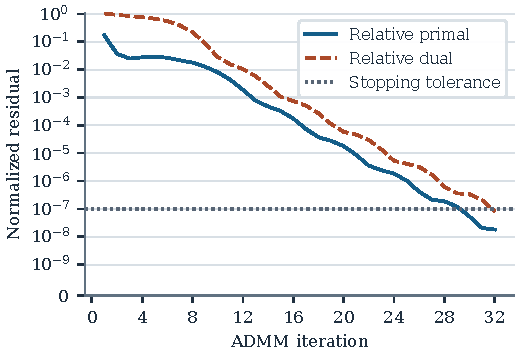
\includegraphics[width=\columnwidth]{convergence.pdf}
 \caption{Residuals for the 10\% trial. The primal curve is $\rho_{\mathrm p}$ from \eqref{eq:primal}, and the dual curve is $\rho_{\mathrm d}$ from \eqref{eq:dual}. The dotted line marks the shared stopping threshold. The vertical scale is linear near zero.}
 \label{fig:convergence}
\end{figure}

The representative solver \RepStatus{} after \RepIterations{} iterations, with terminal primal and dual residuals $\RepPrimal$ and $\RepDual$ (Fig.~\ref{fig:convergence}). Across the main experiment, \MainConverged{} of \MainTrialCount{} runs meet the stopping rule in \MainMinIterations{}--\MainMaxIterations{} iterations, with mean wall times of \MeanPcaMs{} ms for SVD and \MeanPcpMs{} ms for PCP. Table~\ref{tab:diagnostics} records iteration ranges, convergence counts, and mean PCP timing by density. The timings are specific to the measured software and processor.

Each ADMM iteration includes an economy SVD with asymptotic cost $O(mn\min(m,n))$ and $O(mn)$ additional elementwise work. The baseline performs one SVD, while the solver repeatedly recomputes singular directions as $S$ and $Y$ change. For these matrices the full spectrum is affordable and makes thresholding straightforward. The cost increases rapidly with both dimensions, especially when the solver requires many more iterations to meet a tight tolerance.

\subsection{Dense Noise Extension}

\begin{table}[!t]
\caption{Dense Gaussian Noise at 10\% Gross Corruption}
\label{tab:noise}
\centering
\small
\setlength{\tabcolsep}{5pt}
\begin{tabular}{@{}rcccc@{}}
\toprule
$\sigma$ & Mean $E_{\mathrm{PCA}}$ & Mean $E_{\mathrm{PCP}}$ & PCP rank & Mean F1 \\
\midrule
\NoiseRows
\bottomrule
\end{tabular}
\end{table}

Table~\ref{tab:noise} shows how the low-rank error, PCP rank, and support scores vary when the observations also contain dense noise. At $\sigma=0.5$, the estimated support has \NoiseFalsePos{} false positives and \NoiseFalseNeg{} false negatives across the trials. The equality constraint encourages the estimator to explain dense perturbations using additional singular directions and nonzero sparse coefficients. Both effects weaken the interpretation of the two components as the clean signal and the gross errors. The dual and primal checks measure optimization progress for the fitted model, while ground-truth metrics measure whether that model recovers the intended components.

In total, \NoiseConverged{} of \NoiseTrials{} noise fits meet the stopping criteria. Mean iteration counts at $\sigma=0.1$ and $0.5$ are \NoiseMildIterations{} and \NoiseHighIterations{}, respectively. The iteration count can vary with the active support and singular spectrum, so it is a poor proxy for statistical recovery under dense noise. Stable PCP \cite{zhou2010} replaces equality with $\fro{M-L-S}\le\epsilon$, allowing an explicit residual budget when the noise scale can be estimated.

\section{Limitations}
The simulations use small square matrices of one rank, one gross-error magnitude, and uniformly scattered corruptions. Real data can have coherent singular vectors, clustered errors, or entire corrupted rows and columns. Those patterns can overlap with the low-rank subspace and undermine identifiability. Experiments with random Gaussian factors also sidestep real signal spectra, where singular values may decay gradually and a strict true rank may be unavailable.

Providing the true rank to SVD isolates its sensitivity to sparse contamination in this study. In applications, a practitioner must choose the rank using validation or an estimate of the signal spectrum. PCP instead chooses a spectrum through nuclear shrinkage, with results depending on $\lambda$ and the model assumptions. The penalty $\mu$ affects the path to convergence, and the stopping tolerance controls the attainable numerical accuracy at a given runtime. Repeated full SVDs limit scalability. In the noise extension, equality-constrained PCP must absorb dense variation into the low-rank and sparse estimates, and the fixed detection threshold offers a limited view of their use in anomaly detection. The study measures variation over finite synthetic samples, and its comparisons are descriptive.

\section{Conclusion}
This study compared known-rank SVD with PCP on paired observations containing sparse, high-amplitude errors. At 20\% corruption the measured mean errors were $\EndPca$ and $\EndPcp$, respectively, and the support comparison counted \CorruptFalsePos{} false positives and \CorruptFalseNeg{} false negatives across the corrupted main trials. These results favor PCP in this regime, with repeated SVDs as its main computational cost. Truncated SVD remains a direct, inexpensive fit for clean matrices with a known rank. For data containing both gross errors and dense noise, an explicit residual budget can better reflect the observation model.

\bibliographystyle{IEEEtran}
\bibliography{references}
\end{document}
